\documentclass{article}
\usepackage[utf8]{inputenc}
\usepackage{amsmath}
\usepackage{amssymb}
\usepackage{color}
\usepackage{graphicx}
\usepackage{float}
\usepackage{physics}
\title{report v0.tex }
\author{Henrik Linder}
\date{\today}
\begin{document}
\maketitle

Given the rates of protein production and decay as 
\begin{equation}
	k_p^{mRNA} = \frac{1}{600}[s^{-1}],\quad k_d = \frac{1}{1800}N_p[s^{-1}],
\end{equation}
we can describe the change in number of proteins $N_p$ as a function of time with the ODE 
\begin{equation}
	\label{eq:protein_ODE}
	\dv {N_p}{t} = k_p^{mRNA}  - k_dN_p .
\end{equation}
By setting $\dv {N_p}{t} = 0 $, we can see that we get a steady state solution when $k_p^{mRNA} = k_dN_p$, or 
\begin{equation}
	\label{eq:steady_state}
	N_p = 3.
\end{equation}


\begin{figure}[H]
	\centering
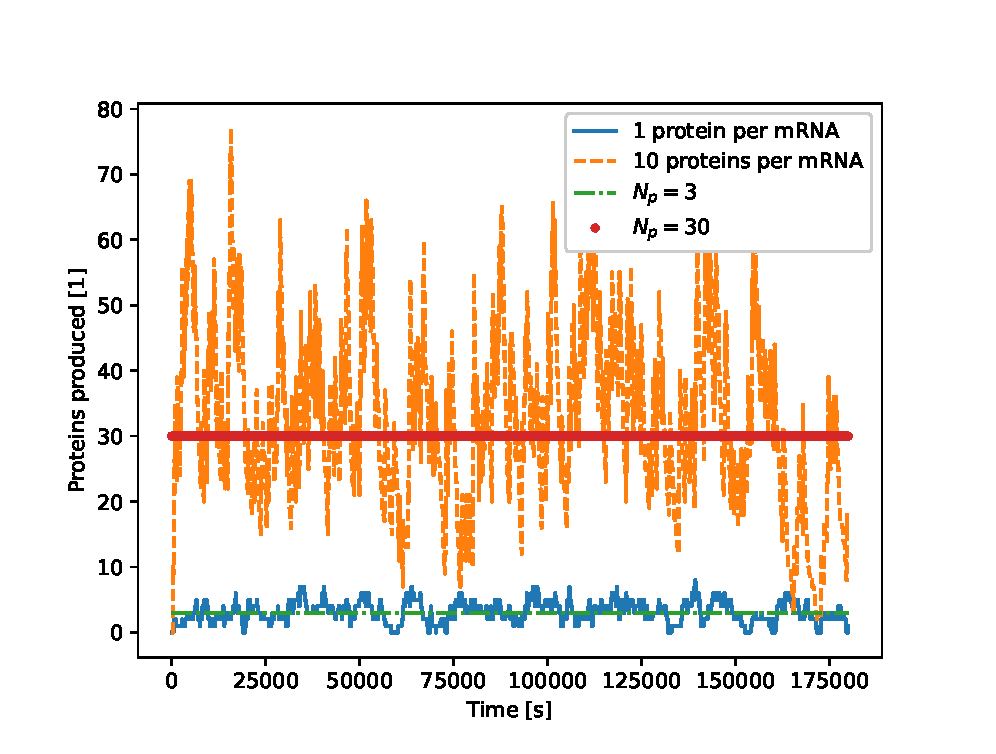
\includegraphics[width = \linewidth]{figs/task1_results_v3.eps}
	\label{fig:task1_results}
\end{figure}

\begin{figure}[H]
	\centering
	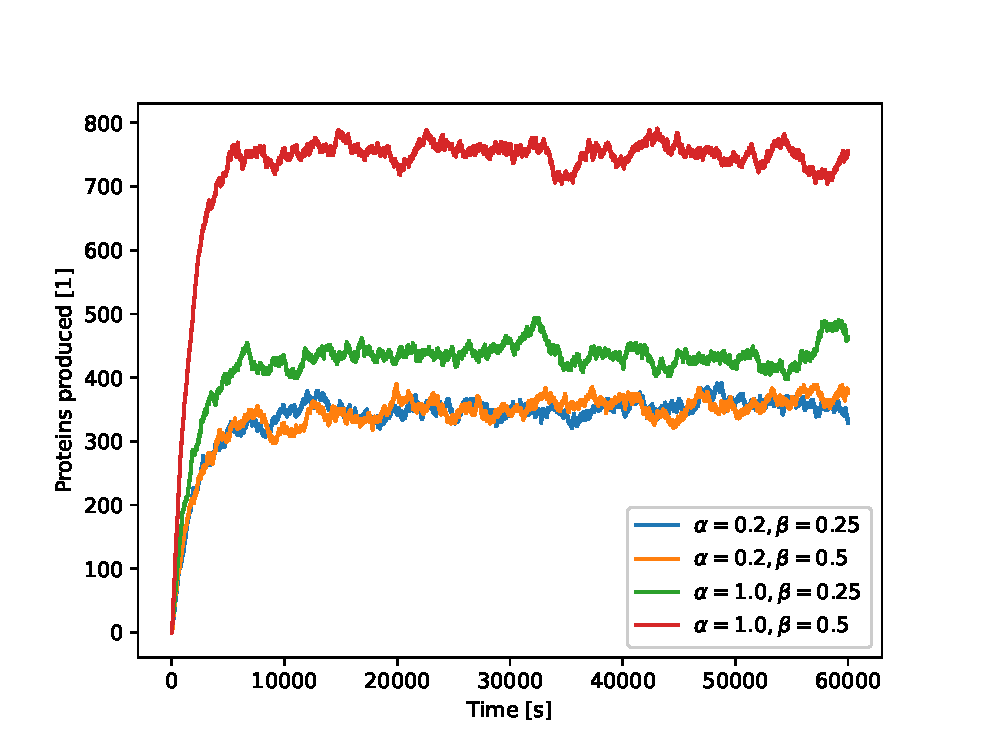
\includegraphics[width = \linewidth]{figs/task2_prot_prod_v4.eps}
	\label{fig:task2_prot_prod}
\end{figure}

\begin{figure}[H]
	\centering
	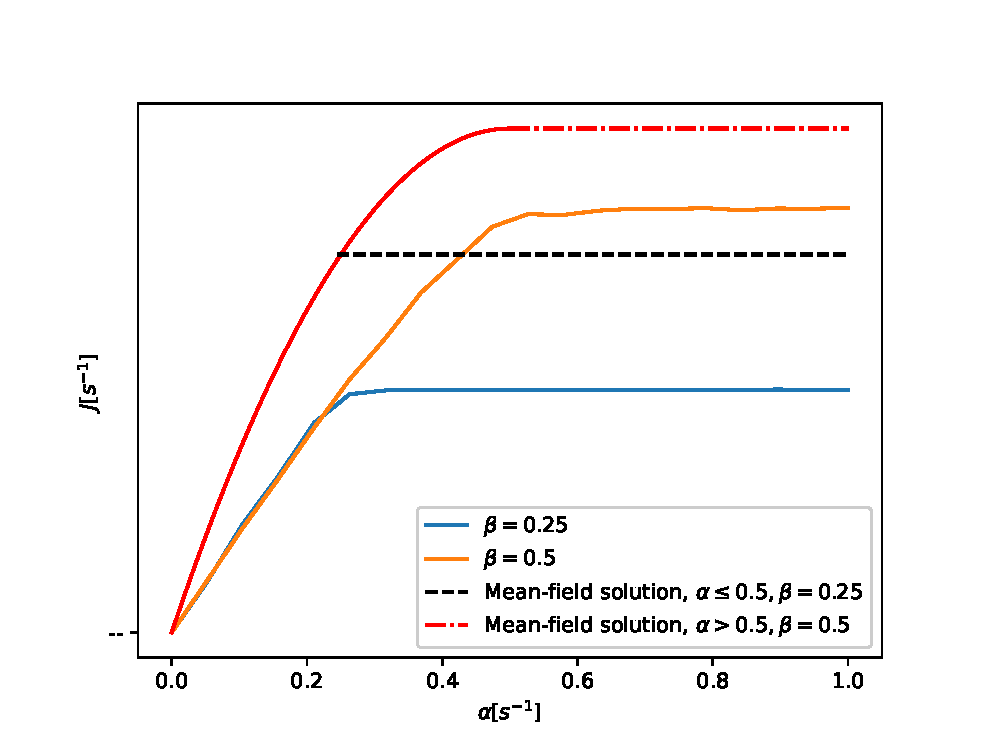
\includegraphics[width = \linewidth]{figs/task2_meanfield_v4.eps}
	\label{fig:task2_mean-field}
\end{figure}


As seen in fig.\eqref{fig:task2_mean-field}, the general behavior of my simulation matches the mean=field approximation. However, it differs quite a bit in total number of proteins produced. 

\section{Task3}
fano1 : 1.1537323139033988,  1.0293234725437235, 1.1255733414025437,  0.9870385180083185


fano cont. : 3.4324503269801925, 2.629365078890865, 2.212654090046395, 2.816569373857693

\begin{figure}[H]
	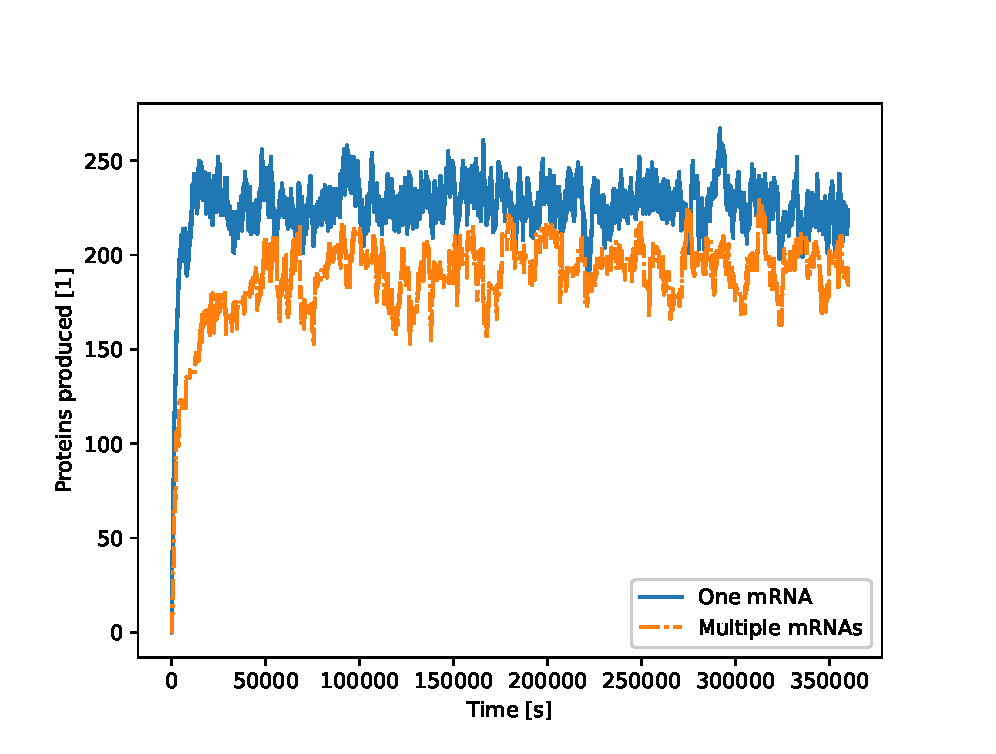
\includegraphics[width=\linewidth]{figs/task3_prot_prod_both_graphs_v1.eps}
	\label{fig:task3}
\end{figure}

As seen in fig.\eqref{fig:task3}, the protein production is actually higher with only one mRNA than it is with multiple. This may be explained by the fact that the 

The fano factor is much higher in the second case. This seems fairly reasonable since we are now adding the mechanism of mRNA decay. It is now antirely possible that an mRNA will be produced, exist for a while, then decay without ever producing a protein. It will however keep ribosomes busy, only releasing them into the free pool upen decay. This may all explain the increased burstiness of the system. 





\section{Task4}
The discrepancy between this model and the real-world behavior of the protein production may be caused by any of a number of factors, but the one that comes to mind is transcription factors (TFs). These affect the transcripton of DNA into mRNA. They react to external signals and bind to the DNA, activating or repressing the transcription of a certain gene

Another mechanism for regulating the protein production is Small RNA regulation. This is where small pieces of RNA attach to the mRNA, blocking the ribosome from passing, effectively stopping the translation of that piece of mRNA. 

Neither of these mechanisms are caught in our model, indicating that we won't be able to reach a realistic real-world behavior for the protein production without modifications. 







\end{document}
